\chapter{Instrument Suite}

* Total mass and power requirement

* What do we want to measure and why? Explain why some instruments were picked and some were discarded (we can use the notes from when we did that in class)

\section{Up-concentration}

\section{Water flow for the instruments} % Figure out a better title?

* Water convection is not enough. We need a pump (peristaltic pump).

\section{Sample handling}

* We need a design, I (Kristian) talked with some other about this, but we need to coordinate with the rest of the groups
   (SMS http://www.esmats.eu/amspapers/pastpapers/pdfs/2008/mumm.pdf)

* Sample rate

* What is under pressure and what is not?

* Order of the instruments

\subsection{Robot Arm} % Rasmus


\section{CTD/ADCP} % Sridhar

* Includes temperature probe

    * We will properly need more around the body of the penetrator

\section{Light sensor}

\section{Gas detection}

\section{XRF}

\section{Lab-in-a-Chip Systems}

\section{pH \& salinity} % Lukas, KSL

* pH
	* Solid state (ISFET)
		* No calibration
		* Measures current flow at different voltages, H+ ions
	* Temperature compensated [5:50] degrees C
		* Response time ~60 s
	* 200 uL, ~20 mW, below 10 mA
	* $\pm$ 0.01 pH
* Salinity can use same instruments using membranes
	* Current flow
* Temperature probe
	* K-type thermal couple

\begin{figure}[htb]
	\centering
	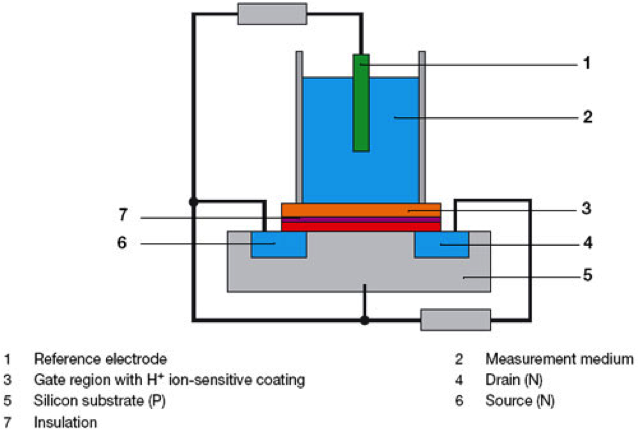
\includegraphics[width=\textwidth]{figures/ISFET.png}
	\caption{TODO: Caption}
	\label{fig:ISFET}
\end{figure}

\section{Camera}

\section{Microscope}
